% !TeX root=main.tex
% دستور زیر باید در اولین فصل شما باشد. آن را حذف نکنید!
\pagenumbering{arabic}

\chapter{مقدمه} \label{ch:intro}
\thispagestyle{empty}


\section{شرح مسأله} \label{sec:sharh}
\paragraph{}
{
    یک عامل برای انجام اقدام مناسب در محیط، باید بتواند محیظ اطراف خودش را درک کند.
    یکی از مهم‌ترین روش‌ها، درک محیط اطراف از طریق دیدن است.
    در سال‌های اخیر، حوزه‌ پردازش تصویر به‌خصوص با وجود ابزاری نظیر یادگیری عمیق پیشرفت چشمگیری داشته‌اند. با توجه به
    وجود داده‌های زیاد در این زمینه‌ها، محققان در حل مسائلی نظیر دسته‌بندی تصاویر
    \cite{He_2016_CVPR}
    ، تشخیص اشیاء
    \cite{Redmon_2016_CVPR}
    و مسائل کاربردی مشابه به خوبی عمل کرده‌اند به‌گونه‌ای که می‌توان ادعا کرد سیستم
    توانایی حل مسئله دسته بندی تصاویر را با دقتی بیشتر از انسان‌ها دارد
    \cite{He_2015_ICCV}!
    با این حال، این مسائل از جمله مسائل ساده هستند و نیاز به درک دقیق اجزاء تصویر و ارتباطات بین آنها ندارند. به
    عبارتی دیگر، به عنوان یک انسان، به سادگی میتوانیم اشیاء موجود در تصویر را تشخیص دهیم و موقعیت آنها را تعیین
    کنیم. 

    یکی دیگر از توانایی‌های مهم و کلیدی عوامل مصنوعی، ارتباط با انسان‌ها است. یک عامل
    مصنوعی باید بتواند با انسان‌ها به ساده‌ترین روش، که همان زبان طبیعی انسان‌هاست،
    با آن‌ها ارتباط برقرار کند. پردازش زبان طبیعی را می‌توان زیرمجموعه‌ای از زبان‌شناسی بین
    انسان‌ها و ماشین‌ها در نظر گرفت. 

    مسائل متفاوتی نظیر عنوان‌نویسی تصاویر، پرسش‌و‌پاسخ تصویری و تولید تصاویر از عناوین
    وجود دارند که پردازش تصویر و پردازش زبان‌ طبیعی را در کنار یکدیگر استفاده کرده‌اند. 
     تا مدتی قبل، پرسش‌وپاسخ تصویری یک اغراق‌نمایی بود تا اینکه یک مجموعه داده در این رابطه منتشر شد. مجموعه
     داده پرسش‌وپاسخ تصویری
     \cite{VQA}
     یک وظیفه جدید را برای حل با خود به همراه آورد که با توجه به پرسش‌ها، نیازمند زیر وظیفه‌های
متفاوت نظیر تشخیص اشیاء
 (تصویر چه شیئی را نشان میدهد؟)
 ، تشخیص مشخصات 
(این شیء چه رنگی دارد؟)
و
موارد مشابه است.

با کاوش کردن مجموعه داده پرسش‌وپاسخ تصویری متوجه‌ تک‌کلمه‌ای بودن پاسخ‌ها می‌شویم که در حال حاضر از الگوریتم‌های دسته‌بندی برای حل این مسئله
استفاده می‌شود. پاسخ دادن به سوال از طریق دسته‌بندی بین کلمات از پیش‌ تعیین شده طبیعی به نظر نمی‌رسد. از آنجایی که هدف هوش مصنوعی حل کردن مسائل
به روش انسان‌ها است و انسان‌ها نیز به صورت جمله به سوالات پاسخ می‌دهند، ارائه دادن پاسخ‌های تک‌کلمه‌ای برای پرسش‌های تصویری اندکی غیر طبیعی به نظر
می‌رسد. از این رو ارائه دادن ساز و کاری برای پاسخ دادن به سوالات به صورت جمله می‌تواند علاوه بر طبیعی کردن مسئله اطلاعات اضافی در اختیار کاربر
قراردهد که منجر به تشخیص بهتر خطاها و رفع ابهامات بسیاری می‌شود.
   }

\section{اهداف پژوهش}
\paragraph{}
{
    هدف اصلی این پژوهش امکان‌سنجی، طراحی، پیاده‌سازی و ارزیابی سیستمی خودکار مبتنی بر روش یادگیری عمیق
    برای پاسخگویی به سوالات مربوط به یک تصویر به صورت جمله است. در این مسئله ورودی یک تصویر به
    همراه یک دنباله‌ای از کلمات به عنوان سوال است. وظیفه سیستم تولید دنباله‌ای از
    کلمات است که بتواند پاسخ سوال مربوط به تصویر را پاسخ دهد. شکل
    \ref{fig:intro_train}
    یک نمونه از پرسش‌وپاسخ تصویر به همراه پاسخ مورد انتظار را نشان می‌دهد. 
    \begin{figure}[H]
        \center{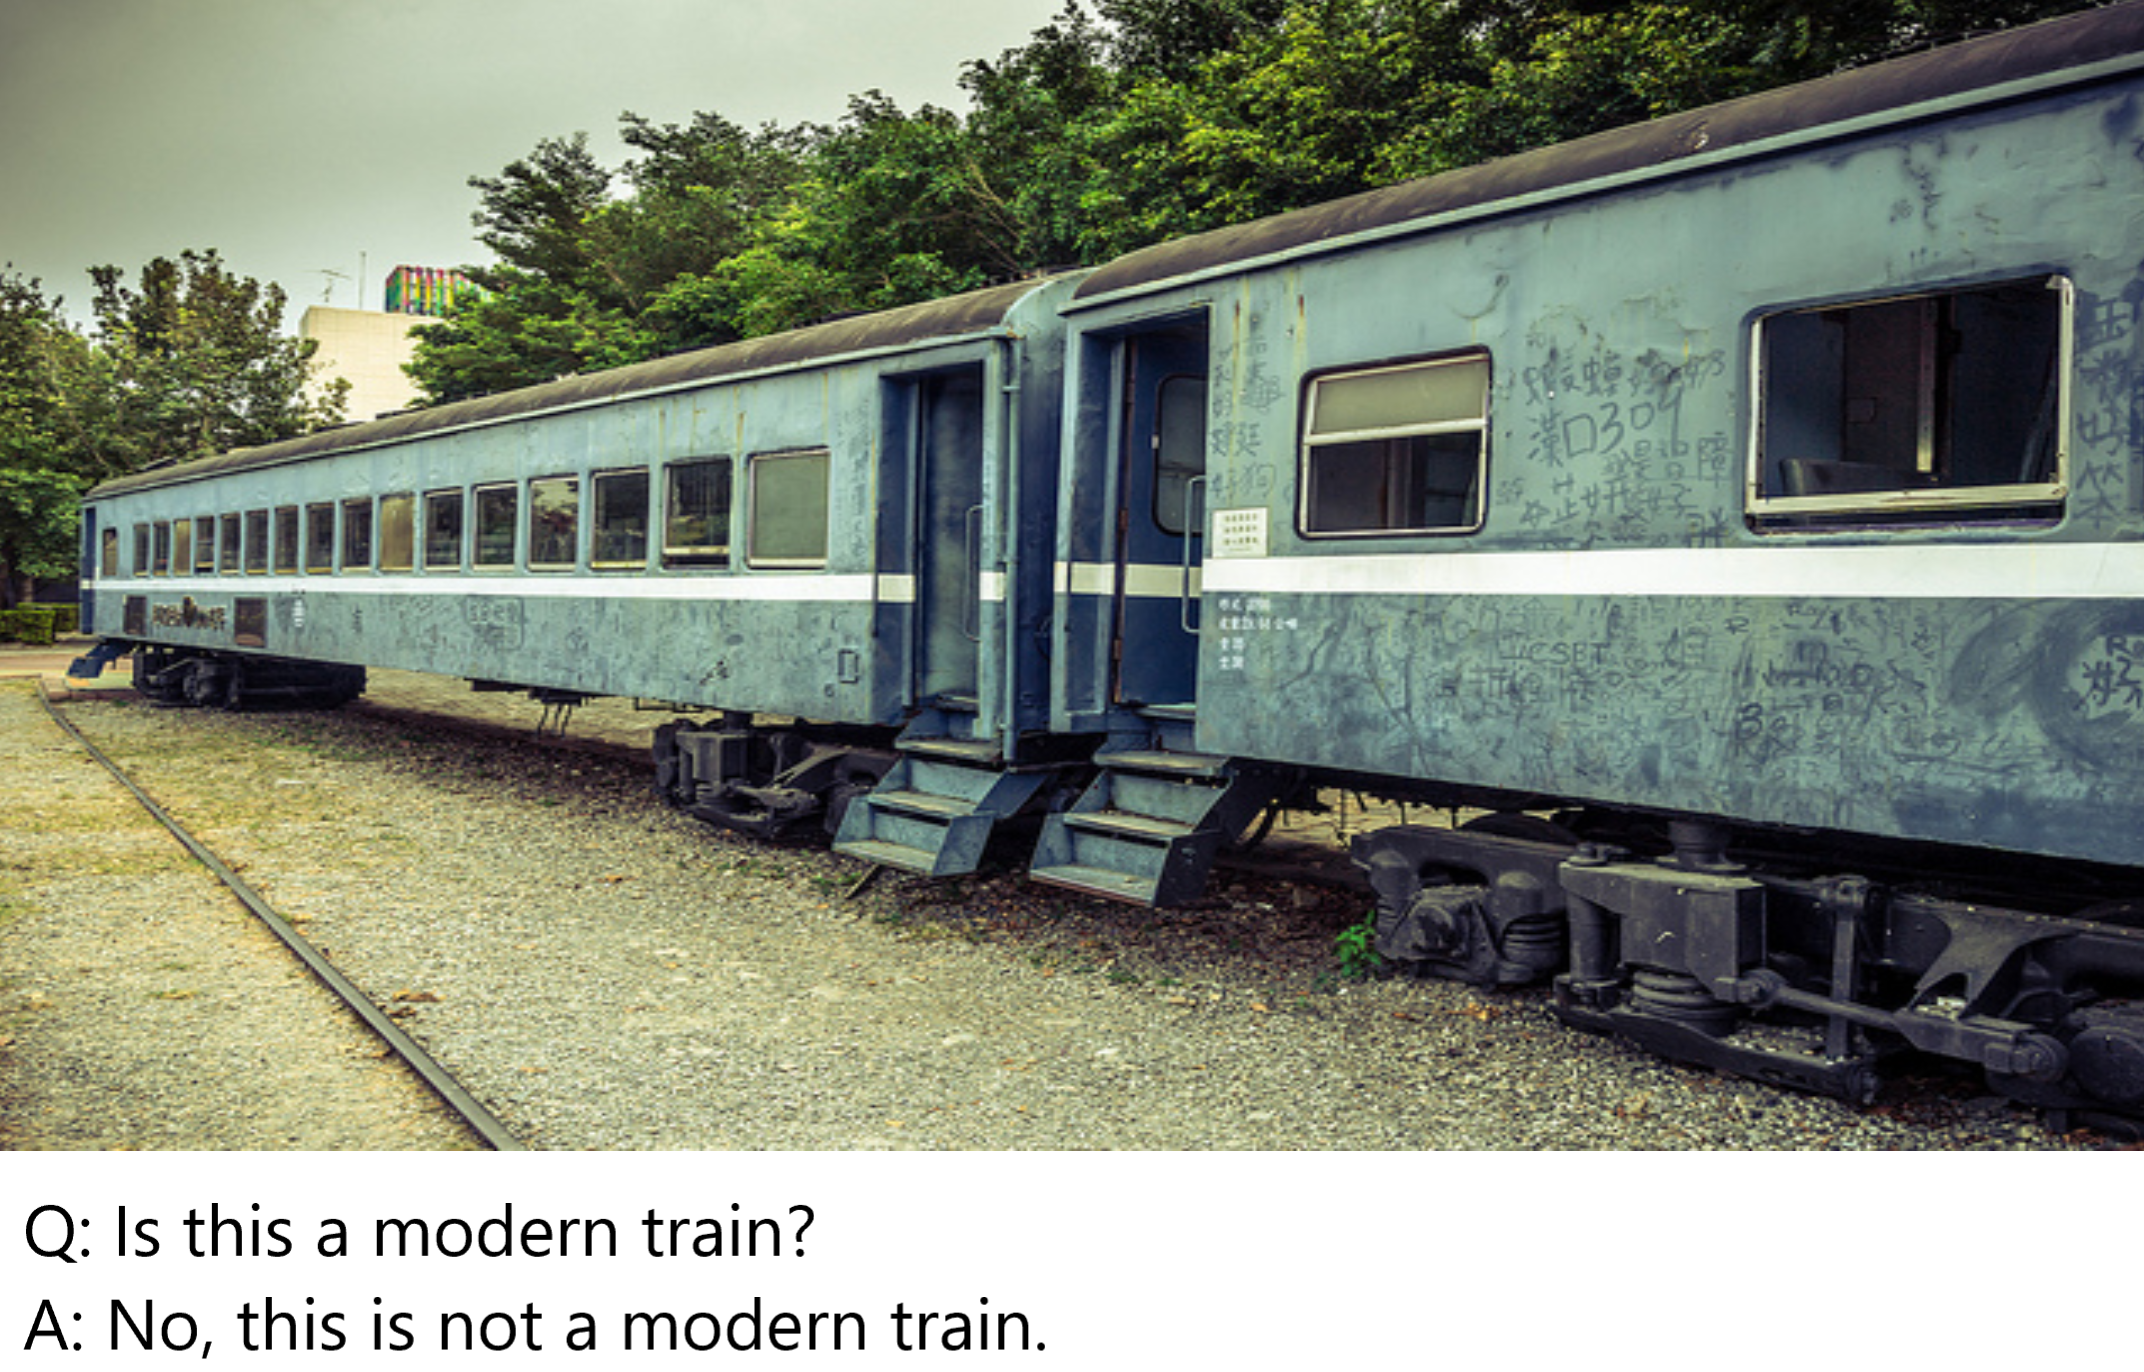
\includegraphics[width=0.7\textwidth]{figs/Intro_objective_train.png}}
        \caption{یک نمونه از جفت پرسش‌ و تصویر همراه با پاسخ مورد انتظار}
        \label{fig:intro_train}
    \end{figure}
}
\section{ساختار گزارش}
\paragraph{}
{
    در این پروژه هدف ارائه 
    روشی نو برای حل مسئله پرسش‌وپاسخ تصویری است. 
    در ابتدا به معرفی مفاهیم پایه استفاده شده در این پژوهش 
    و سپس به معرفی روش‌ها و کارهای مرتبط پرداخته‌ 
    خواهد شد. پس از آن به معرفی 
    روش و ارزیابی آن پرداخته شده است. در انتها نتیجه‌گیری و 
    کارهای آینده معرفی می‌شوند. 


}